We built and uses an Entity System as an underlying game engine framework.
The idea behind an entity system is that objects should be treated as pure aggregations of data containers, with game logic being separated from objects all together. Instead of having deep class hierarchies and chained method calls, logic for managing specific components is batched on all such components in the system. This provides some advantages over other approaches such that the architecture becomes more flexible and extendable. It is clearer how to build functionality and especially where. Another advantage from the batching is the possibility of much higher performance (maximizing caching and minimizing cache misses) as well as simplifying parallelism of logic processing.

\subsection{Entity System}
An Entity System consists of three main parts: Entities, Components and Systems.
An Entity is simply a label or identifier of an object. A Component is a pure data containers, and each entity has a collection of none to several different components. A System consist of logic for working with primarily one, but sometimes several, components. So, an object is an entity label and a collection of components that belong to it. The object is updated by different systems performing tasks on the components. A example used in this project is seen in figure \ref{fig:EntityComponentSystemExample}.
\begin{figure}[H]
  \centering
  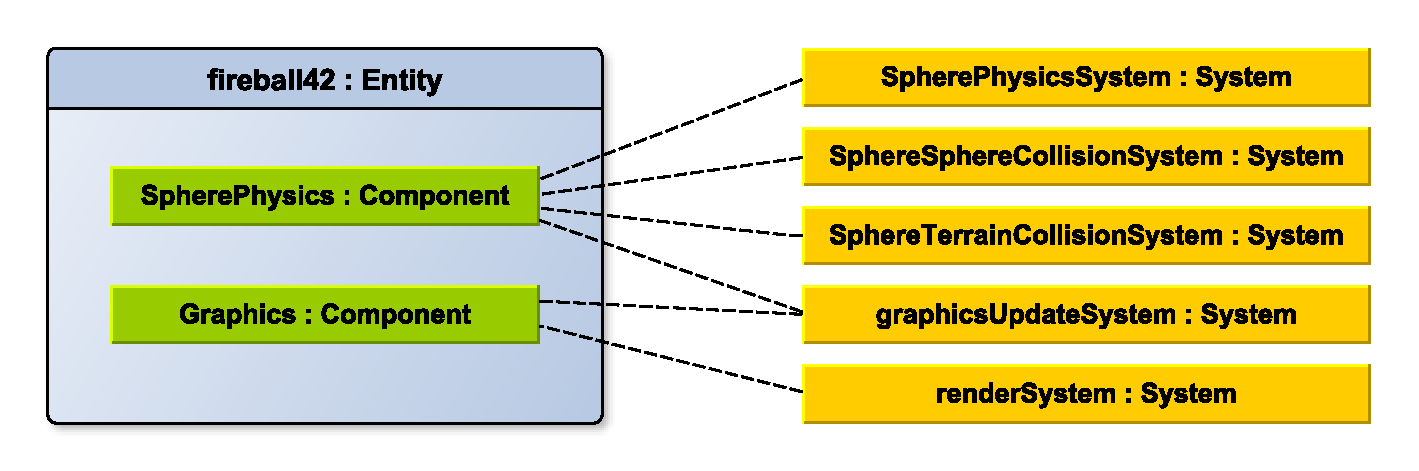
\includegraphics[width=0.9\linewidth]{images/EntityComponentSystemExample.eps}
  \caption{Caption}
  \label{fig:EntityComponentSystemExample}
\end{figure}
(TODO: reformulera och skriv nedan mer flytande och omarbetat)\\
* The idea behind: Systems perform on ALL components of a certain type, which is fetched from the EntityManager.\\
* Our system allows for components to require other components. This means that systems which work on multiple components can be proven to always work by fetching the component which require the others. The require check is performed at compile time and code is generated to handle the specific requirement-tree specified. The program writes part of itself to be maximum efficient and robust, by specifications by the developer in the source code.\\
* Easy to use (a natural work flow of what goes where and how to solve problems. minimal overhead to use the system), easy to maintain, easy to extend, extremely efficient, trivial to parallelize calculations, verifies consistency at compile time...

\subsection{Rendering}

\subsection{Physics}
The physics used in this game is divided into three systems, all three processing all \textit{SpherePhysics} components in the Entity System. The physics is limited to 3D sphere physics as well as the interaction between spheres and a terrain mesh.\\
\\
\subsubsection{SpherePhysics}
SpherePhysics is a component dedicated to physics data, its content is seen in the code below.
\begin{lstlisting}
 struct SpherePhysics : public Component<> {
    const std::string getName() override { return "SpherePhysics"; }

    float mass;                     // m            (Positive)
    float elasticity;               // epsilon      (Between 0 and 1)
    float friction;                 // friction     (Between 0 and 1)
    float momentOfInertia;          // For a sphere: 6/12*m*radius^2
    float gravitationalConstant;    // g            (Positive. in Sweden at sea level: 9.82)

    QVector3D force;                // F = ... external events ...
    QVector3D linearMomentum;       // P = Integral( F, dt );
    QVector3D velocity;             // v = P / m;
    QVector3D position;             // x = Integral( v, dt );

    QVector3D torque;               // T = ... external events ...
    QVector3D angularMomentum;      // L = Integral( T, dt );
    QVector3D angularVelocity;      // w = L * Inverse(I)
    QQuaternion angularVelocity2;   // w = L * Inverse(I)
    QQuaternion rotation;           // r = Integral( w, dt );

    float radius;                   // Radius of the sphere
    QVector3D collisionVector;      // The sum of the vectors from all collisions

 };
\end{lstlisting}

\subsubsection{SpherePhysicsSystem}
The sphere physics are based on the physics lab, with a generalization to 3D and using quaternions as the representation for rotation. The system require the current time step $dt$. which is used as the integration step in the Euler-forward integration used. This was sufficient for our needs, with no more advanced integration schemes necessary.\\
\\
The spheres are affected by external forces and torques, which then updates the rest of the physical states. At the end, any forces and torques has been handled and are set to zero, and finally the ever present gravitational force is added.

\subsubsection{SphereSphereCollisionSystem}
The sphere-sphere collision handling are based on the physics lab, with a generalization to 3D. The collision is handled by reversed impulse. Collisions give rise to torque, making he collisions seem very realistic.

\subsubsection{SphereTerrainCollisionSystem}
The sphere-sphere collision handling uses the terrains height and normal at the bottom of the sphere. It is otherwise similar to the SpherePshereCollisionSystem apart from that the terrain is considered to have infinite mass. A normal force is applied to the object to minimize noise from the gravity force. A friction force can be used if a more realistic collision is desirable. In our demonstration it isn't used since we had a limited amount of fire balls, so the fewer that got stuck on land the longer the volcano could spew out new fire balls.
